\subsection{Local Semi-Honest RM-VOLE Performance}
\label{sec:module-mvole-performance}

We evaluate a local semi-honest prototype for rank-one module VOLE (RM-VOLE). The target functionality is
\[
  P_0: x \in R_p,\ Z_0 \in R_{p^m}, \qquad
  P_1: \Delta \in \mathbb{F}_{p^m},\ Z_1 \in R_{p^m},
\]
with correctness relation
\[
  Z_0 + Z_1 = \Delta \cdot x.
\]
The implementation represents elements of \(\mathbb{F}_{p^m}\) and \(R_{p^m}\) by \(m\) base-field coordinates over \(\mathbb{F}_p\), so the verifier checks the coordinate image of the relation.

We compare three measurements. First, \texttt{--MODULE\_MVOLE\_PPRF} is the intended shared-path vector-valued PPRF RM-VOLE setup: each regular sparse block expands one tree and derives all \(m\) coordinates from the shared leaves, so the expanded leaves per sparse vector are \(N\). Second, \texttt{--MODULE\_MVOLE\_COORD\_PPRF} is a semantic coordinate-wise baseline for the same RM-VOLE functionality: it runs a separate scalar regular-block PPRF for every coordinate, so the scalar-coordinate expanded leaves per sparse vector are \(mN\). Third, \(m\cdot\texttt{QA\_VOLE}\) is only a generic scalar cost proxy; it is not semantically equivalent because independent QA-SD VOLE instances produce independent right vectors, whereas RM-VOLE produces one shared right vector \(x\).

All timings are medians of three runs on a 64-vCPU Intel Xeon Platinum 8269CY system. The code is built from commit \texttt{27ec607}. The prototype is local: it does not include network transport, base OT, silent setup serialization, or malicious-security checks. No WHT parallel optimization is added in this baseline.

\begin{table}[t]
\centering
\small
\begin{tabular}{rrrrrrrrrrr}
\toprule
\(N\) & \(t\) & \(m\) & block & vec/N & coord/N & vector (s) & coord (s) & coord/vector & \(m\cdot\)QA (s) & QA proxy/vector \\
\midrule
1024 & 8 & 8 & 128 & 1 & 8 & 0.000872 & 0.000989 & 1.13$\times$ & 0.144226 & 165.40$\times$ \\
4096 & 16 & 16 & 256 & 1 & 16 & 0.006894 & 0.007266 & 1.05$\times$ & 0.294669 & 42.74$\times$ \\
16384 & 32 & 16 & 512 & 1 & 16 & 0.028522 & 0.044866 & 1.57$\times$ & 0.267189 & 9.37$\times$ \\
65536 & 64 & 16 & 1024 & 1 & 16 & 0.126704 & 0.194964 & 1.54$\times$ & 0.372547 & 2.94$\times$ \\
262144 & 128 & 16 & 2048 & 1 & 16 & 0.632057 & 0.662134 & 1.05$\times$ & 0.909234 & 1.44$\times$ \\
65536 & 64 & 32 & 1024 & 1 & 32 & 0.242992 & 0.254451 & 1.05$\times$ & 0.745094 & 3.07$\times$ \\
262144 & 128 & 32 & 2048 & 1 & 32 & 1.182721 & 1.176052 & 0.99$\times$ & 1.818467 & 1.54$\times$ \\
\bottomrule
\end{tabular}
\caption{Median local runtime for shared-path vector RM-VOLE, coordinate-wise scalar RM-VOLE, and the \(m\cdot\texttt{QA\_VOLE}\) proxy. The coordinate-wise baseline is semantically equivalent to RM-VOLE but does not share PPRF tree work across coordinates.}
\label{tab:module-mvole-semantic-baseline}
\end{table}

\begin{table}[t]
\centering
\small
\begin{tabular}{rrrrr}
\toprule
\(N\) & \(m\) & setup (\%) & expand (\%) & verify (\%) \\
\midrule
1024 & 8 & 22.2 & 49.3 & 4.0 \\
4096 & 16 & 20.7 & 49.1 & 4.0 \\
16384 & 16 & 20.8 & 51.2 & 4.1 \\
65536 & 16 & 19.5 & 49.4 & 3.6 \\
262144 & 16 & 16.9 & 48.7 & 3.0 \\
65536 & 32 & 25.2 & 49.8 & 3.8 \\
262144 & 32 & 21.2 & 51.0 & 3.1 \\
\bottomrule
\end{tabular}
\caption{Percentage runtime breakdown for \texttt{--MODULE\_MVOLE\_PPRF}. Expansion consists of the P0 and P1 row-wise WHT work.}
\label{tab:module-mvole-breakdown}
\end{table}

Figure~\ref{fig:module-mvole-runtime} plots total runtime against \(N\), while Figure~\ref{fig:module-mvole-coordinate-speedup} shows the speedup of the shared-path vector PPRF path over the coordinate-wise RM-VOLE baseline. For the tested settings, vector RM-VOLE is faster than the coordinate-wise semantic baseline for most points, with a median speedup ranging from roughly parity to about \(1.6\times\). The benefit is larger when the setup materialization is a meaningful fraction of total time; when \(N\) is large, row-wise WHT expansion dominates and the advantage from sharing PPRF paths is partially hidden. Against the generic \(m\cdot\texttt{QA\_VOLE}\) proxy, vector RM-VOLE remains faster throughout the measured grid, but this comparison should be read as a cost proxy rather than a functionality-equivalent baseline.

\begin{figure}[t]
  \centering
  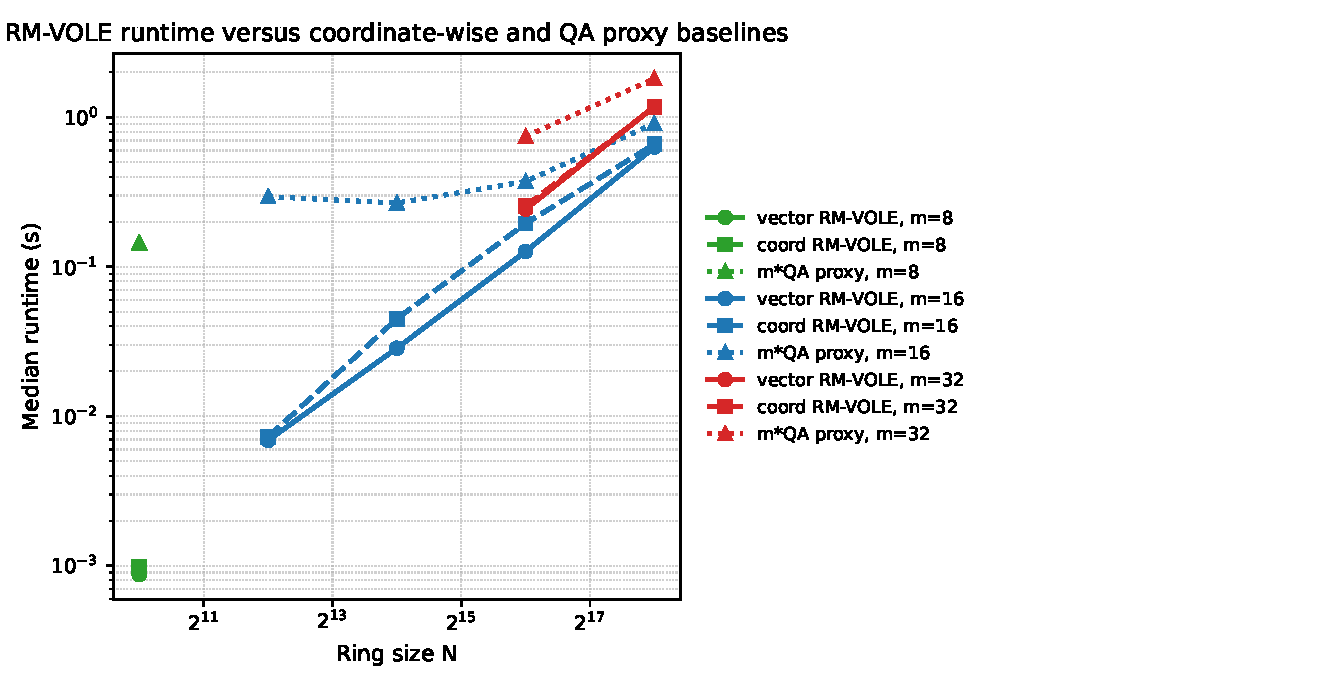
\includegraphics[width=.78\linewidth]{docs/module_mvole_paper_figures/runtime_vs_N.pdf}
  \caption{Median runtime for shared-path vector RM-VOLE, coordinate-wise scalar RM-VOLE, and the \(m\cdot\texttt{QA\_VOLE}\) proxy.}
  \label{fig:module-mvole-runtime}
\end{figure}

\begin{figure}[t]
  \centering
  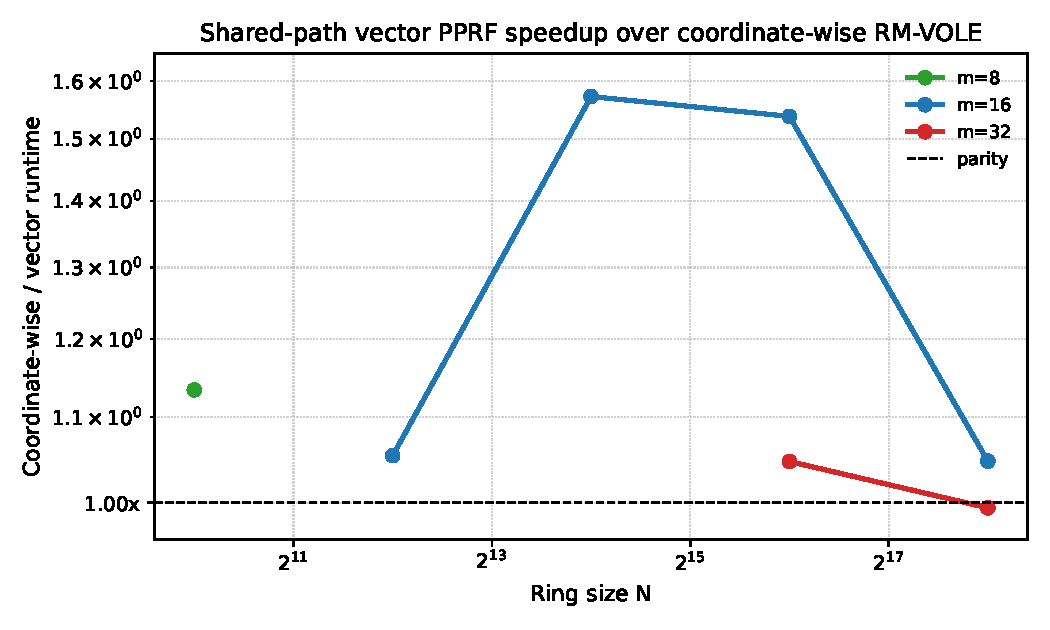
\includegraphics[width=.70\linewidth]{docs/module_mvole_paper_figures/speedup_vs_coordinate_baseline.pdf}
  \caption{Speedup of shared-path vector-valued PPRF RM-VOLE over the semantic coordinate-wise scalar PPRF RM-VOLE baseline.}
  \label{fig:module-mvole-coordinate-speedup}
\end{figure}

\paragraph{Takeaway.}
The shared-path vector-valued PPRF reduces the setup leaf expansion from \(mN\) scalar-coordinate leaves to \(N\) shared leaves per sparse vector. This gives a clean semantic win over the coordinate-wise RM-VOLE baseline in setup, and a moderate end-to-end win whenever setup is not completely hidden by WHT expansion. The dominant cost in the larger settings is P0/P1 expansion, especially the row-wise WHTs, so the next optimization target is batched or parallel row-wise WHT, or direct WHT-domain share generation.
